\chapter{Fundamentos Teóricos}

% https://medium.com/analytics-vidhya/automated-keyword-extraction-from-articles-using-nlp-bfd864f41b34
% https://course.spacy.io/
% https://medium.com/qu4nt/reducir-el-n%C3%BAmero-de-palabras-de-un-texto-lematizaci%C3%B3n-y-radicalizaci%C3%B3n-stemming-con-python-965bfd0c69fa
% https://towardsdatascience.com/topic-modeling-and-latent-dirichlet-allocation-in-python-9bf156893c24
% https://medium.com/@datamonsters/text-preprocessing-in-python-steps-tools-and-examples-bf025f872908
% https://towardsdatascience.com/end-to-end-topic-modeling-in-python-latent-dirichlet-allocation-lda-35ce4ed6b3e0
% http://datamining.dc.uba.ar/datamining/files/Tesis/TesisGastonLiberman.pdf
% https://towardsdatascience.com/tf-idf-for-document-ranking-from-scratch-in-python-on-real-world-dataset-796d339a4089



\section{Minería de texto}

Se debe definir primero conceptos básicos que son clave para hablar de minería de textos 
como dato, información, conocimiento y minería de datos, para lograr un mejor entendimiento y
contextualizar al lector desde una primera instancia.

Dato es un conjunto discreto de valores, por ejemplo:  Mateo, Sistemas, 10 . Información es el conjunto de
datos procesados y que tienen un significado (relevancia, propósito y contexto) dado por el observador,
como puede ser, Mateo estudio 10 semestres   de ingeniería de sistemas. Luego, el conocimiento será la capacidad de
transformar la información y la experiencia de las personas en la toma de decisiones sobre una acción.
En el mundo de las tecnologías de la información, los datos son almacenados normalmente en bases de
datos y su volumen puede llegar a ser muy grande, a partir de esto surge la minería de datos para ayudar
a la comprensión de los contenidos en dicho almacenamiento. Las bases de datos tienen una estructura
y un esquema de organización conocido o estructurado, luego a partir de ellas se trata de adquirir conocimiento de datos
originales, lo que hace más fácil la extracción de información.

La minería de texto (text data mining TDM) es una aplicación de la minería de datos \cite{Hearts2013} y
consiste en descubrir o hallar, a partir de cantidades de información no estructurada el conocimiento del
cual no existe ningún registro escrito. La información no estructurada es aquella que no está contenida
en un “almacén” (base de datos), de forma organizada para luego ser encontrada y utilizada fácilmente
para distintos propósitos, lo que dificulta su extracción. Esta información puede estar representada en
textos como los mensajes de correo electrónico, presentaciones en power point, documentos en word,
mensajes instantáneos (Twitter, WhatsApp), software de colaboración (conferencias de video, salas de
chat), entre otros; o se encuentra de forma no textual en imágenes de formato JPEG, archivos de audio
MP3, correo de voz, etc. 

La principal característica de la minería de texto es que trabaja con base en el lenguaje natural. Este
lenguaje es el que hablamos los humanos todos los días, es espontáneo, no es artificial y no ha sido
programado de ninguna manera.

Se enfoca en el descubrimiento de patrones interesantes o sucesos recurrentes, su objetivo es descubrir
tendencias, desviaciones y asociaciones en la gran cantidad de información textual disponible. Algunas
aplicaciones de los sistemas de minería de textos son la identificación y re direccionamiento del
contenido de e–mails; los sistemas de vigilancia tecnológica, análisis de información en artículos y libros,
búsqueda relevante de contenido en artículos, etc.

Por su parte, Ronen Feldman, y James Sanger la describen como un proceso intensivo de conocimiento
en el que un usuario interactúa con una colección de documentos en el tiempo, utilizando un conjunto
de herramientas de análisis; además, busca extraer información útil de una fuente de datos a través de la 
identificación y exploración de patrones interesantes. En ella las fuentes de datos son las colecciones de documentos y
los patrones interesantes se encuentran en textos generalmente no estructurados \cite{feldman2007advanced}.

En \cite{viera2017tecnicas} la minería de texto proviene en gran parte de las investigaciones en minería de datos y,
por lo tanto, tienen similitudes en su arquitectura de alto nivel; por ejemplo, 
ambos sistemas se basan en rutinas de preprocesamiento, algoritmos para descubrir patrones 
y la capa de elementos de presentación que contienen herramientas
de visualización para mejorar la navegación en los conjuntos de respuestas.


Feldman y Sanger  \cite{feldman2007text}, también señalan las diferencias entre minería de datos y minería de texto.
Para ellos, en la primera, los datos se guardan en formatos estructurados, y gran parte de su preprocesamiento
se centra en la depuración y normalización de los datos, así como en crear un gran número de uniones de tablas. 
En contraste, en la minería de texto, el preprocesamiento se enfoca en reconocer y extraer características 
representativas para documentos en lenguaje natural. Tales características pueden ser palabras clave relevantes, 
identificación de nombres de personas, organizaciones, etcétera. El objetivo del preprocesamiento es transformar 
datos no estructurados que se encuentran en la colección de 
documentos en un formato intermediario estructurado más explícito.

I.H Witten \cite{witten2016data}, explica la diferencia entre la minería de datos y la minería de texto,
indicando que, en la primera, se procura extraer información implícita, previamente desconocida y
potencialmente útil a partir de un gran volumen de datos. En la segunda, la información a ser extraída
se encuentra escrita en el texto en forma clara y explícita. Sin embargo, el problema principal para el usuario
es la dificultad de tener que acceder y leer grandes volúmenes de documentos textuales en formato digital que están disponibles
en la actualidad para fines informativos, estratégicos o de recreación.

Michael W. Berry y Jacob Kogan \cite{berry2010text}, a su vez, afirman que los mayores temas estudiados en la minería de texto
son la extracción de palabras clave, clasificación, agrupamiento, extracción de nombres y entidades, detección de anomalías y 
tendencias y flujos de texto. Cada uno de esos temas forma parte de un subárea de la minería de texto.

En la subárea de resumen de texto, la salida del sistema de minería de texto es el resumen de características que
se destacan (trechos relevantes dentro de los documentos) en un gran acervo textual. Otra subárea de la minería de
texto es la clasificación, en la que cada instancia representa un documento y las clases son los asuntos tratados.
Así, los documentos se clasifican según las palabras que aparecen dentro de los mismos utilizando diferentes técnicas 
de la minería de texto \cite{witten2016data}.

El agrupamiento de documentos es otra subárea más de la minería de texto, donde son reunidos de acuerdo con 
criterios de similitud entre las palabras que se encuentran. La principal característica de esta técnica es que
no existen categorías predefinidas, sin embargo, esto permite que sea definido el número de grupos que se desea
crear para el conjunto de documentos que se procesarán \cite{viera2017tecnicas}.

La minería de textos cuenta con una metodología propia para llevar a cabo el proceso de extracción de
información. Esta metodología puede ser entendida como el proceso mediante el cual se llevan a cabo
una serie de tareas ordenadas orientadas para la consecución de tres objetivos principales:\\ \\
1. Establecimiento del corpus (conjunto de textos)\\
2. Transformación de documentos no estructurados a estructurados\\
3. Extracción del conocimiento.

\section{Bag of Words (Bolsa de palabras, BoW)}
El modelo bag-of-words (bolsa de palabras, BoW) en el procesado de lenguaje
natural es un método popular para representar documentos, que ignora el orden de las
palabras. El modelo BoW permite un modelado basado en diccionario, y cada
documento parece una bolsa (de ese modo no se considera el orden), que contiene
algunas palabras del diccionario,cada palabra constituye una posición de un vector y el valor corresponde 
con el número de veces que ha aparecido \cite{pardo2009aplicacion}.

Cada documento se representa por una serie de términos, un término es una palabra o grupo de palabras útiles
para describir el contenido del documento,todos los términos son independientes entre sí, lo que implica que puedo
calcular la importancia de cada término en un documento independientemente de los otros 
(la independencia no es cierta, pero en la práctica funciona).
El peso wij de un término ti en un documento dj es proporcional a la importancia de ese término.

Para complementar el proceso de bolsa de palabras existen técnicas para reducir el
número de palabras en el conjunto de documentos, tales como stemming o raiz, lexeme o lematización, eliminar palabras muertas\cite{gomesGarcia}.


\textbf{Stop words (Palabras muertas )}

Las stop words son palabras frecuentes dentro de una cadena de texto. Generalmente, son
palabras comunes tales como el, la, y, pero, etc. En inglés, sería: the, and, but, etc. Estas
palabras ayudan a formar ideas, pero no suelen tener valor individualmente.

\textbf{Lematización}

La lematización relaciona una palabra flexionada o derivada con su forma canónica o lema. 
Y un lema no es otra cosa que la forma que tienen las palabras cuando las buscas en el diccionario.
por ejemplo  canto, cantas, canta, cantamos, cantáis, cantan son distintas formas (conjugaciones) de un mismo verbo (cantar).
Y que niña, niño, niñita, niños, niñotes, y otras más, son distintas formas del vocablo niño. Así que la lematización encuentra estas 
diferencias y agrupa todas estas variantes en un mismo término.

La lematización es un proceso clave en muchas tareas prácticas de procesamiento de lenguaje natural (PLN), pero tiene dos costos. Primero,
es un proceso que consume recursos (sobre todo tiempo). Segundo, suele ser probabilística, 
así que en algunos casos obtendremos resultados inesperados \cite{LinoAlbertoUrdanetaFernandez}.



\textbf{Stemming (Raíz)}

Stemming es el proceso de reducir las palabras de una cadena de texto a su raíz.
Estas raíces son la parte invariable de palabras relacionadas sobre todo por su forma. Por ejemplo,
las palabras intelligence e intelligent se reducen a la raíz intellig.

El stemming es mucho más rápido desde el punto de vista del procesamiento que la lematización. 
También tiene como ventaja que reconoce relaciones entre palabras de distinta clase. Podría reconocer,
por ejemplo, que picante y picar tienen como raíz pic-. En otras palabras,
el stemming puede reducir el número de elementos que forman nuestros textos.
Y eso, en muchos casos, es lo que buscamos.

Como desventaja pueden “recortar” demasiado la raíz y encontrar relaciones entre palabras que realmente no existen,
un stemmer sólo procesa una palabra y desconoce el contexto en donde se ubica dicha palabra,
suele ser una buena solución cuando no importa demasiado la precisión y se requiere de un procesamiento eficiente


\section{Term Frequency — Inverse Document Frequency (Término de Frecuencia - Frecuencia inversa del documento,TF-IDF)}

Resumiendo lo dicho en \cite{aggarwal2012mining} esta es una técnica para cuantificar una palabra en documentos, generalmente calculamos un peso para cada 
palabra que significa la importancia de la palabra en el documento y el corpus. Este método es una técnica ampliamente utilizada
en recuperación de información y minería de texto.

Aumenta a medida que aumenta el número de apariciones de esa palabra en el documento,
se equilibra por el peso o frecuencia del termino en la colección 
de documentos, permitiendo manejar el hecho de que algunas palabras son mas comunes que otras ,
es decir incorpora un factor de frecuencia inversa de documento que atenúa el peso de los términos que ocurren con mucha frecuencia en la colección de documentos e 
incrementa el peso de los términos que ocurren pocas veces.\\

%%Matemáticamente:\\
TF-IDF = Frecuencia de término (TF) * Frecuencia de documento inversa (IDF)  \\ 

Terminología:\\ \\ t - término (palabra)  \\
d - documento (conjunto de palabras) \\
N - recuento de corpus \\
corpus - el conjunto total de documentos \\

\textbf{Term Frequency (Término de Frecuencia , TF)}

Mide la frecuencia de una palabra en un documento. Esto depende en gran medida de la longitud del documento y de
la generalidad de la palabra, por ejemplo, una palabra muy común como "fue" puede aparecer varias veces en un documento. 
pero si se toma dos documentos, uno con 100 palabras y otro con 10000 palabras. Hay una alta probabilidad de que la palabra
común como "fue" pueda estar presente más en el documento redactado de 10000. 
Pero no se puede afirmar que el documento más largo es más importante que el documento más corto. 
Por esta razón exacta, TF  normaliza  el valor de frecuencia, dividiendo la frecuencia 
con el número total de palabras en el documento.\\

tf(t,d) = número de veces que aparece t en d/ número de palabras en d \\


Cuando estamos vectorizando los documentos, verificamos el recuento de cada palabra.
En el peor de los casos, si el término no existe en el documento, ese valor de TF particular será 0 y,
en otro caso extremo, si todas las palabras en el documento son iguales, entonces será 1. 
El valor final de la normalización El valor de TF estará en el rango de [0 a 1]. 0, 1 inclusive.


\textbf{Document Frequency, Frecuencia de Documento, DF}

 Mide la importancia del documento en todo el conjunto de corpus, esto es muy similar a TF.
 La única diferencia es que TF es un contador de frecuencia para un término t en el documento d, 
 DF es el recuento de ocurrencias del término t en el conjunto de documentos N. En otras palabras, 
 DF es el número de documentos en los que la palabra está presente . Consideramos una ocurrencia si el término consiste
 en el documento al menos una vez, no necesitamos saber la cantidad de veces que el término está presente.\\
 
df (t) = aparición de t en documentos


\textbf{Inverse Document Frequency, Frecuencia de Documento Inversa, IDF}


IDF es el inverso de la frecuencia del documento que mide la informatividad del término t. 
Cuando calculemos IDF, será muy bajo para las palabras más frecuentes, como las palabras muertas
(porque las palabras muertas como (es, la, el, a, para,...,etc) están presentes en casi todos los documentos,  N / df dará un valor muy bajo a esa palabra ) 
Esto finalmente da un peso relativo. \\

idf(t) = N/df \\


Ahora hay algunos otros problemas con las IDF, en caso de un gran corpus, digamos 10000, el valor de las IDF explota. 
Entonces, para amortiguar el efecto, tomamos el registro de IDF.
Durante el tiempo de consulta, cuando aparece una palabra que no está en vocabulario, 
el df será 0. Como no podemos dividir por 0, suavizamos el valor agregando 1 al denominador.\\

idf(t) = log(N/(df + 1)) \\

Finalmente, al tomar un valor multiplicativo de TF e IDF, obtenemos el puntaje TF-IDF \\

tf-idf(t, d) = tf(t, d) * log(N/(df + 1))


\section{Topic Modeling Latent Dirichlet Allocation (
Modelado de temas, LDA)}

El modelado de tópicos es una técnica que suele aplicarse para el agrupamiento y
clasificación de datos en una colección de textos \cite{ahmed2012timeline}.

previamente a la explicación del algoritmo 
como se define en \cite{DescubrimientoPatrones}, explicamos los conceptos de palabra, documento, corpus y tópico.
Una palabra es una unidad básica de información discreta, que en este contexto se
define como un elemento de un vocabulario indexado V.
Un documento es una secuencia de N palabras denotadas por w = (w1, w2, ..., wN ),
donde wn es la n-ésima palabra en la secuencia.
Un corpus es una colección de M documentos denotada por: D = {w1, w2, ..., wM}.
Un tópico es una distribución de probabilidad sobre un vocabulario fijo.
El proceso de generación de cada documento en la colección se desarrolla como se
describe a continuación:\\ \\
1. Elegir una distribución aleatoria sobre los tópicos.\\
2. Para cada palabra en el documento: \\
\subitem a) Elegir aleatoriamente un tópico. 
\subitem b) Dado ese tópico, elegir una palabra probable (generada en el paso 1). \\

Este modelo refleja la intuición que los documentos contienen múltiples tópicos.
Cada documento muestra los tópicos en distinta proporción (paso 1), cada palabra en
cada documento se extrae de uno de los tópicos (paso 2b), donde el tópico seleccionado
es elegido de la distribución por documento sobre los tópicos (paso 2a).

Todo proceso generativo basado en probabilidades se basa en la existencia de variables
no observables en la colección. Para obtener información sobre estas es necesario
inferir la distribución conjunta entre eventos conocidos y eventos latentes. Se puede
obtener esta información a través del uso de distribuciones condicionales de eventos
ocultos, dado que ya se conocen las distribuciones de eventos observables. En el modelo
LDA, los eventos observables son la aparición de palabras en los documentos; y las
variables ocultas son todas aquellas que caracterizan la estructura de tópicos de una
colección de documentos.
En modelado probabilíıstico generativo, se tratan los datos como provenientes de
un proceso generativo que incluye variables ocultas. Se ejecuta el análisis de los datos
utilizando una distribución conjunta para computar la distribución condicional de las
variables ocultas, dadas las variables observadas.\\

El proceso generativo se define como:

\subitem 1. Para cada tópico k, definir una distribución sobre las palabras  $\phi$k $\sim$ Dir$( \alpha )$.
\subitem 2. Para cada documento d,
\subsubitem a) Definir un vector con proporciones de tópico $\theta$d $\sim$ Dir$(\beta)$.
\subsubitem b) Para cada palabra i
\subsubitem \quad 1) Definir una palabra wd, i $\sim$ Mult$(\theta d)$, zd,n $\in$ \{1, ..., K\}.
\subsubitem \quad 2) Definir una palabra wd, i $\sim$ Mult($\phi$zd,i ), wd,i  $\in$ \{1, ..., V \}.\\
\subitem Dada la siguiente notación:\\
\subitem Dir es una distribución Dirichlet
\subitem Mult es una distribución Multinomial
\subitem $(\beta)$1:K, son los tópicos
\subitem $(\beta)$k es una distribución de palabras para el tópico k
\subitem $\theta$d, es la proporción de tópicos para el documento d-ésimo
\subitem $\theta$d,k es la proporción del tópico k en el documento d
\subitem zd es la asignación de tópicos para el documento d-ésimo
\subitem zd,n es la asignación de tópicos para la n-ésima palabra en el documento d
\subitem wd son las palabras observadas para el documento d
\subitem wd,n es la n-ésima palabra en el documento d \\


A partir de esta notación, se puede definir el proceso generativo de documentos a
través de la distribución conjunta de variables observables y ocultas; como se describe en la figura \ref{ecuacion1} \\

\begin{figure}[H]
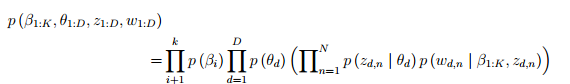
\includegraphics[width=1\textwidth]{ec1}
\caption{Ecuación de distribución conjunta \cite{DescubrimientoPatrones}}
\label{ecuacion1}
\end{figure}


Esta distribución especifica una serie de dependencias. La asignación del tópico zd,n
depende de la proporción del tópico $\theta$d por documento.
Las palabras observadas wd,n dependen de la asignación de tópico zd,n y de todos
los tópicos $(\beta)$1:K. Estas dependencias definen el modelo LDA.
Una vez definido el modelo que representa las relaciones entre los tópicos, los documentos
y las palabras existentes en un corpus, para que este sea de utilidad es necesario
calcular las distribuciones condicionales de la estructura de los tópicos, dada la colección
de documentos. Esta distribución es lo que se llama como posterior. La definición
posterior se desprende de la ecuación descrita en la figura \ref{ecuacion1} y se detalla en la figura \ref{ecuacion2}:\\

\begin{figure}[H]
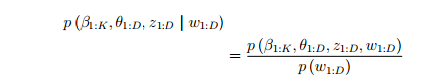
\includegraphics[width=1\textwidth]{ec2}
\caption{Ecuación de distribución conjunta alternativa \cite{DescubrimientoPatrones}}
\label{ecuacion2}
\end{figure}

El numerador es la distribución conjunta de todas las variables aleatorias, que pueden
ser fácilmente calculadas para cualquier conjunto de variables ocultas. El denominador
es la probabilidad marginal de las observaciones, que es la probabilidad de ver
el corpus observado bajo cualquier modelo de tópicos. En teoría, puede computarse
sumando la distribución conjunta de cualquier posible combinación de la estructura
de tópicos ocultos. Como para muchos problemas bayesianos, no se puede computar la
probabilidad posterior por el denominador, conocido como “evidencia”. Los algoritmos
de modelado de tópicos producen una aproximación de la ecuación \ref{ecuacion2} formando una
distribución alternativa a lo largo de la estructura latente de tópicos que se adapta para
acercarse a la real posterior.


\section{Word2vec}

Con el objetivo de la automatización del resumen de textos, se puede utilizar una
variedad de técnicas, como Hidden Markov Models , técnicas de grafos, y acercamientos
sobre distribución de probabilidades \cite{heuer2015semantic}. Propuesto por Sahlgren \cite{sahlgren2005methods} (hipótesis distributiva) las palabras con un significado similar
ocurren en similares contextos . Esto implica que el significado de las palabras se
puede inferir por su distribución contextual. Bruni y otros \cite{bruni2014multimodal} demuestran
que esta teoría tiene múltiples raíces teóricas estudios de lingüística , lexicografía
y filosofía. El objetivo de la semántica distributiva es encontrar una representación, por
ejemplo, un vector, que aproxime el significado de una palabra. La hipótesis distributiva
propone que los términos con propiedades de distribución similares tienen un significado
similar \cite{sahlgren2005methods}.
Uno de los desafíos de la semántica distributiva es computar vectores de palabras
que sean representaciones adecuadas de las palabras. Se utilizan varias arquitecturas
para computar tales vectores de palabras. Tradicionalmente, los vectores de palabras
se entrenan como parte de un lenguaje de modelado de redes neuronales. De acuerdo
con Mikolov, las redes neuronales artificiales pueden pensarse como una proyección
no lineal de los datos \cite{mikolov2013efficient}. Las redes neuronales artificiales (RNA)
son un sistema para el tratamiento de la información, cuya unidad de procesamiento
básica está inspirada en la neurona humana \cite{de1998aplicacion}. para ampliar más conceptos en redes neuronales ver 
\cite{rajasekaran2003neural}.


Word2vec fue desarrollado por Mikolov, Sutskever, Chen, Corrado y Dean en Google
y publicado en 2013 \cite{mikolov2013efficient}. Word2vec es una herramienta que implementa
dos formas de computar representaciones de palabras: continuous bag-of-words
(CBOW) y continuous skip-gram (CSG) .
Word2vec toma un corpus como entrada y produce vectores de palabras como resultado.
Primero construye un vocabulario desde los textos de entrenamiento y luego
aprende una representación vectorial de palabras, En \cite{goldberg2014word2vec} se ha demostrado que las representaciones vectoriales de palabras aprendidas
por los modelos word2vec tienen significados semánticos y conceptuales. El vector de palabras resultante puede
usarse como variables en aplicaciones de procesamiento de lenguaje natural y aprendizaje automático.
La ventaja que presenta Word2vec es su utilización de modelos de redes neuronales que
entienden el significado semántico de las palabras.
Las arquitecturas que se utilizaron previamente a CBOW y CSG fueron RNA alimentadas
hacia adelante (Feedforward Neural Net Language Model -NNLM) , y Redes
neuronales con conexiones recurrentes (Recurrent Neural Net Language Model -
RNNLM).
El modelo de lenguaje probabilístico de red neuronal feedforward (NNLM) se compone
de capas de entrada, capa de proyección, capa oculta y capas de salida. En la
capa de entrada, N palabras anteriores se codifican utilizando una de-codificación V ,
donde V es el tamaño del vocabulario. La capa de entrada es entonces proyectada a
una capa P proyección que tiene dimensión N * D, utilizando una matriz de proyección
compartida, donde D es la dimensionalidad de las palabras en el espacio. Como sólo N
entradas están activas en un momento dado, la composición de la capa de proyección
es una operación relativamente barata.
El modelo RNNLM no tiene una capa de proyección, sólo entrada, oculta y salida.
Lo que tiene especial este modelo es la matriz recurrente que conecta la capa oculta a
sí misma, usando conexiones demoradas en el tiempo. Esto permite al modelo recurrente
formar una memoria de corto plazo.
Continuous Bag-of-Words Model es similar a feedforward NNLM, donde la capa
oculta no lineal se remueve y la capa proyectada se comparte para todas las palabras,
por lo tanto, todas las palabras se proyectan en la misma posición (sus vectores se
promedian). Se llama a esta arquitectura modelo bag-of-words, porque el orden de las
palabras en la historia no influencia la proyección.
Continuous Skip-gram Model es similar a CBOW, pero en vez de predecir la palabra
basada en el contexto, trata de maximizar la clasificación de una palabra basada en
otra palabra en la misma oración. Se utiliza cada palabra como una entrada en un
clasificador log-lineal con una capa continua proyectada, y predice palabras con un
cierto rango antes y despúes de la actual palabra.
Aumentando el rango mejora la calidad de los vectores de palabras resultantes, pero
también incrementa la complejidad computacional. Desde que las palabras más distantes
están usualmente menos relacionadas con la palabra actual que aquellas cercanas a
ella, se les da menos peso a las palabras distantes muestreando menos de esas palabras
en los ejemplos de entrenamiento.
Para reducir el número de categorías y mejorar la eficiencia, la primera opción de
los investigadores fue el agrupamiento (clustering). La idea principal fue agrupar las
palabras similares en una clase y luego utilizarla para representar cada palabra. Los
vectores computados por Word2vec contienen información semántica. En word2vec la
mayor contribución es que se puede con exactitud calcular la similitud entre palabras
utilizando esos vectores \cite{yuan2014new}. 
Para ello, se pueden obtener las palabras similares calculando la similitud coseno
como medida de distancia. Se pueden agrupar estas palabras similares en la misma
clase computando la similitud coseno luego de definir el número de grupos. Luego de
obtener los grupos, se pueden contar las palabras que aparecen en él y sumar el número
como un valor de la dimensión correspondiente. El vector obtenido es la variable del
documento. Este vector integra la Información semántica de las palabras similares. Los
vectores de Word2vec se pueden utilizar como atributos para tareas de procesamiento
de lenguaje natural supervisadas, como clasificación de documentos, reconocimiento de
entidades nombradas y análisis de sentimiento.
Por ejemplo, en \cite{yuan2014new} se utilizaron dos conjuntos de datos. Luego del
pre-procesamiento , se armó un corpus.
Cada cinco palabras contiguas se tomó como una ventana, y se introdujo en
Word2vec. Se definió la dimensión del vector en 200. Se pudieron obtener n * 200
vectores despúes de entrenar la red neuronal, donde n es el número de palabras. Tomando
estos vectores, se utilizaron para calcular la similitud coseno cada dos palabras.
Luego, las palabras más similares se agruparon en un cluster. En el diseño de los experimentos,
se definió el número de clusters en 50. Luego se etiquetaron los clusters en cada
palabra y se computaron los features (atributos) de los documentos a través de estos
clusters. Se inicializaron los features en un vector de dimensión d * 50, donde d es el
número de documentos y cada columna representa un cluster. Si una palabra pertenece
al i-ésimo cluster aparece en el documento, el correspondiente feature sumaría +1 en
la i-ésimo dimensión. Con esta metodología, se obtuvieron todos los vectores de features.
Se dividieron los datos en entrenamiento y testing, y se entrenó  un clasificador SVM
(Support Vector Machine, ver en \cite{tong2001support}. Se compararon los resultados
de esta metodología versus LDA y TF-IDF . En ambos conjuntos de
datos, el resultado utilizando word2vec fue superior al resto.

\textbf{Modelo continuo de bolsa de palabras (Continuous Bag-of-Word Model)}



Partiendo del modelo básico de \cite{mikolov2013efficient},
 \cite{goldberg2014word2vec} supone que solo se considera una palabra por contexto, lo que significa que el modelo predecirá una palabra objetivo dada una palabra de contexto, que
es como un modelo de bigrama. La idea es tratar las palabras alrededor de una palabra central como su contexto. E.g., {“El”, “gato”, “se”, “sobre”, “el”, “sillón”} viene a ser el contexto de
la palabra “sentó” \cite{cardellinoproyecto}.

La Figura \ref{redcbow} muestra el modelo de red bajo la definición de contexto simplificada.

\begin{figure}[H]
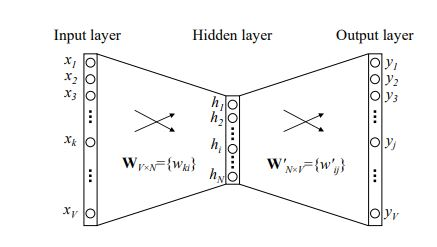
\includegraphics[width=1\textwidth]{redcbow}
\caption{Un modelo CBOW simple con solo una palabra en el contexto \cite{goldberg2014word2vec}}
\label{redcbow}
\end{figure}



 En la configuración, el tamaño del vocabulario es V, y el tamaño de la capa oculta es N. Las unidades de las capas adyacentes están completamente conectadas. La entrada es un vector ''one-hot encoding'', lo que significa que para un
palabra de contexto de entrada, solo una de V unidades, {x1, · · ·, xV}, será 1, y todas las demás unidades serán 0.
Según \cite{cardellinoproyecto} se toma como punto inicial el vocabulario V = w ^{(1)}$, w^{(2)}$, . . . , w^{(m)}$ (|V | = m). A cada palabra w^{(i)}$ se la representa con un vector one-hot x^{(i)}$ \in {R^{m}$}. Para definir los parámetros a actualizar, creamos dos matrices W^{(1)}$  \in R^{m \times n}$ y W^{(2)}$  \in R^{n \times m}$. Donde n es la dimensión final que queremos para los vectores aprendidos  .

Continuando la propuesta de \cite{cardellinoproyecto} La matriz W^{(1)}$ está formada por m filas u^{(i)}$ \in R^{n}$ , estas representan el vector codificado de entrada de la palabra w^{(i)}$ . A su vez, la matriz de salida W^{(2)}$ se conforma de m columnas v^{(j)}$ \in R^{n}$ , que representan el vector codificado de salida de la palabra w^{(j)}$ . Es decir, por cada palabra del vocabulario, se aprenden dos vectores de palabras.

El modelo de CBOW consta de los siguientes pasos:

\begin{itemize}
	\item Se busca obtener la palabra central w^{(i)}$ dado el contexto. (w^{(i - C)}$, . . . , w^{(i -1)}$, w^{(i+1)}$, . . . , w^{(i+C)}$).
	\item Se genera los vectores one-hot para cada una de las palabras del contexto (x^{(i - C)}$ , . . . , x^{(i - 1)}$, x^{(i+1)}$, . . . , x^{(i+C)}$ ).
	\item Obtenemos los vectores codificados de entrada por cada vector one-hot (u^{(i - C)}$ = x^ {(i - C)}$^{T}$ W^{(1)}$, . . . , u^{( i - 1)}$ = x^{ (i -1)}$^{T}$ W^{(1)}$, u^{(i+1)}$ = x^{ (i+1)}$^{T}$ W^{(1)}$, . . . , u^{(i+C)}$ = x^{(i+C)}$^{T}$ W^{(1)}$).
	\item Se busca la media de los vectores para obtener un vector\\  h =(u^{(i - C)}$+u^{(i - C+1)}$+···+u^{ (i+C)}$ ) /(2C) .
	\item Y lo transformamos en un vector de probabilidades mediante y^{'}$ = softmax(z).
	\item Queremos que las probabilidades  y^{'}$^{(i)}$ , sean iguales a las probabilidades correctas, y^{(i)}$, i.e,el vector one-hot de la palabra w^{(i)}$.
\end{itemize}

Una vez se sabe la funcionalidad del modelo en caso de tener los valores correctos para W^{(1)}$ y W^{(2)}$, se pregunta cómo aprender dichas matrices. Si se observa, se entiende que las matrices forman una red neuronal que se entrena mediante retro-propagación y cuya arquitectura se muestra en la Figura  \ref{redcbow}. 


\textbf{Modelo de Skip-Gram}

SkipGram es el otro modelo propuesto por Mikolov \cite{mikolov2013efficient}. Difiere de CBOW ya que busca, dada una palabra central llamada contexto (e.g., “sentó”), predecir las palabras que conforman su alrededor (e.g, “El”, “gato”, “se”, “sobre”, “el”, “sillón”).
 Similar CBOW, solo cambian los papeles de los vectores codificados de entrada (que pasa a ser uno solo) y los vectores codificados de salida (que pasan a ser varios)\cite{goldberg2014word2vec}.
Las matrices siguen siendo las mismas. El modelo skip-gram, trabaja de la siguiente manera:

\begin{itemize}
\item Buscamos obtener las palabras (w^{ (i - C)}$ , . . . , w^{(i - 1)}$, w^{(i+1)}$, . . . , w^{(i+C)}$ ), dada la palabra central w ^{(i)}$ .
\item Generar el vector one-hot para la palabra de entrada x^{(i)}$ .
\item Obtener el vector codificado de entrada u^{(i)}$ = x^{( i)^{T}$}$W^{(1)}$ .
\item Como es un solo vector de entrada, no hay necesidad de obtener la media. Definimos h = u^{(i)}$ .
\item Se genera 2C vectores de puntaje (z^{(i - C)}$ , . . . , z^{(i - 1)}$, z^{(i+1)}$, . . . , z^{(i+C)}$ ) con z^{(j)}$ = h^{(T)}$W^{(2)}$
\item Se Transforma cada vector de puntaje en un vector de probabilidades,  y^{'}$^{(j)}$ = softmax(z^{(j)}$).
\item Se quiere que los vectores de probabilidad generados  (  y^{'}$^{(i - C)}$ , . . . ,   y^{'}$^{(i - 1)}$ ,  y^{'}$^{ (i+1)}$ , . . . ,   y^{'}$^{(i+C)}$ ), sean iguales a las probabilidades verdaderas, (y^{(i - C)}$ , . . . , y^{(i - 1)}$, y^{(i+1)}$, . . . , y^{(i+C)}$ ), i.e. de los vectores one-hot por cada palabra de salida.
\end{itemize}

Similar al modelo CBOW, se calcula los valores de las matrices W^{(1)}$ y W^{(2)}$ . Nuevamente las matrices forman una red neuronal que se entrenara mediante retro-propagación y cuya topología se muestra en la Figura \ref{redskg}.

\begin{figure}[H]
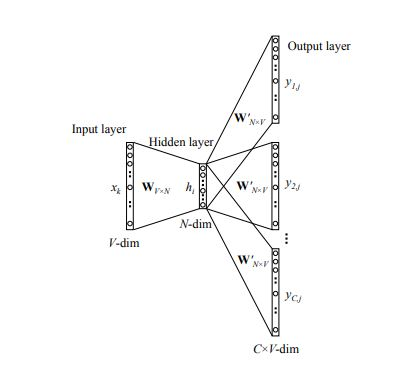
\includegraphics[width=1\textwidth]{redskg}
\caption{Topología del modelo Skip-Gram \cite{mikolov2013efficient}}
\label{redskg}
\end{figure}

\section {Document Embeddings con Doc2Vec}

Doc2Vec es una técnica para representar documentos como vectores de longitud fija y baja dimensionaldad (conocidos también como document embeddings).
Fue creado por Mikolov y Le \cite{le2014distributed} en 2014 en su paper “Distributed Representations of Sentences and Documents”. Mikolov, es también uno de los autores del modelo antes mencionado Word2Vec \cite{mikolov2013efficient}.


En las pruebas realizadas en \cite{capello2018sistema} se ve como Doc2vec supera a otros métodos,
Doc2vec es una extensión del modelo Word2vec.  

La representación vectorial de Doc2vec se crea usando alguno de los dos algoritmos o modelos incorporados: Continuous Bagof-Words (CBOW) y Skip-Gram.

Doc2Vec, tiene dos algoritmos para obtener los embeddings: PV-DM (Paragraph Vector - Distributed Memory) y PV-DBOW (Paragraph Vector - Distributed Bag of Words). Cada uno surge de la extensión de los algoritmos wor2vec anteriormente descritos, respectivamente.

\textbf{PV-DM}

El modelo PV-DM está basado en el modelo Word2vec CBOW, la cual consiste en una red neuronal con tres capas: una de entrada (input), una oculta (o hidden layer) y una de salida (ouptut); con ella se aprenden representaciones de palabras dado un determinado contexto.

El método a Doc2Vec (PV-DM, Figura \ref{pvdm}) extiende de CBOW, se agregan nodos de entrada adicionales (contexto adicional), un nodo por cada documento identificados inicialmente por los ids: 0, 1, …, |Corpus|-1. Por lo tanto, se extiende aún más la capa de entrada.

\begin{figure}[H]
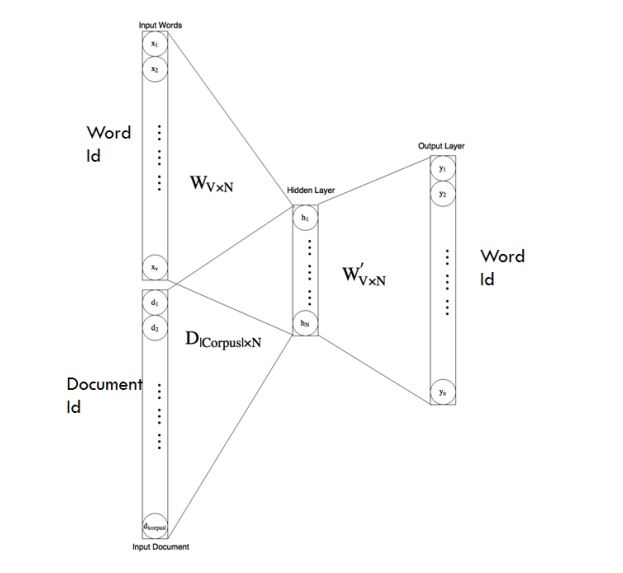
\includegraphics[width=1\textwidth]{pvdm}
\caption{Red neuronal ilustrativa en PV-DM \cite{capello2018sistema}}
\label{pvdm}
\end{figure}


Después se ejecuta el algoritmo de retro-propagación de la misma forma descrita en CBOW, con el id correspondiente al id del documento con el cual se está entrenando, para el cual pertenece la oración seleccionada.  Una vez finalizado el proceso de entrenar contextos de palabras junto con el id del documento, se terminan obteniendo en la matriz D document embeddings y en la matriz W word embeddings. Mediante medidas de similitud, como la del coseno, se hallan los vectores más semejantes a uno fijado, tanto en W, como en D; dependiendo del interés.

\textbf{PV-DBOW}

El modelo de Distributed Bag of Words (DBOW) es la contraparte al modelo PV-DM. El modelo DBOW no tiene en cuenta las palabras de contexto en la entrada, pero obliga al modelo a predecir palabras muestreadas aleatoriamente del documento (dentro de la “ventata”), en la salida. En el ejemplo que se aprecia en la
Figura  \ref{doc2veceje} el modelo aprende mediante  la predicción de 4 palabras muestreadas. Por tanto, para aprender el vector de documento, se muestrean 4 palabras de (the, cat, sat, on, the, mat), repitiendo este proceso un gran número de veces análogamente al anterior proceso, para varias muestras en el documento.

\begin{figure}[H]
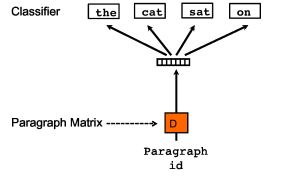
\includegraphics[width=1\textwidth]{doc2veceje}
\caption{ PV-DBOW simplificado \cite{le2014distributed}}
\label{doc2veceje}
\end{figure}




%https://nlp.cic.ipn.mx/Publications/2010/Generacion%20de%20grafos%20conceptuales.pdf

%http://www.scielo.org.mx/scielo.php?pid=S0187-358X2017000100103&script=sci_arttext&tlng=en

\section{K-means (K-M)}

En \cite{manning2010introduction} afirman que el objetivo del algoritmo k-media
es minimizar el error cuadrático medio de la distancia Euclidiana de los documentos con respecto al centroide del grupo 
al cual hacen parte. El centro de un agrupamiento es definido como la media o centroide de los documentos que están en un agrupamiento.

Según \cite{witten2016data} a La métrica para ver si un centroide representa bien a sus miembros del grupo,
es la suma residual cuadrática (SRC), 
que es la sumatoria de la distancia cuadrática de todos los vectores con relación al centroide.
El SRC es la función objetiva del k-media y el objetivo es minimizarla,el algoritmo de k-media no garantiza que 
será alcanzado el mínimo global al utilizar la función objetiva,por ejemplo, si la muestra posee 
muchos valores atípicos no se ajustará bien a ninguno de los agrupamientos.

Otro problema del k-media es que debido a la selección aleatoria inicial de los centroides, 
los agrupamientos resultantes pueden variar mucho en calidad y finalmente el método k-media no sirve
para descubrir agrupamientos con formas no convexas o agrupamientos con diferentes tamaños \cite{wang2011new}.



\section{Antecedentes}

Las organizaciones mayormente disponen de información en documentos de texto no estructurado ,
se encuentran tipificados de esa manera ya que la información contenida en el documento no tiene ningún orden de estructura, ésta
información tiene mayor riesgo de no ser encontrada por los buscadores, pues no contiene parámetros establecidos que proporcionen
la información que se está buscando y sea presentada al usuario, por esta razón la minería de texto adquiere un rol importante
ya que es el proceso de extraer información interesante y conocimiento no trivial de textos no estructurados incluyendo tecnologías 
para extracción de información, seguimiento de temas, generación automática de resúmenes de textos, categorización,
agrupamiento , relaciones entre conceptos , visualización y respuesta automática de preguntas .  

\cite{troyano2003identificacion} describe los principales enfoques de extracción y reconocimiento de NER (entidades con nombre ) , 
el NER desempeña un papel muy importante en diversos problemas relacionados a la búsqueda automática y la categorización de textos.
 
En \cite{figuerola2004algunas} se propone un nuevo método para la caracterización de documentos que sin importar el idioma en el que el 
documento esté escrito, permite extraer el conjunto de palabras clave más adecuado. Su funcionamiento se basa en una Red Neuronal, que
luego de ser entrenada es capaz de decidir para cada término del documento si se trata de una palabra clave o no. El ingreso del documento a la Red Neuronal implicó la definición de una representación numérica adecuada que permite medir la participación de un término dentro del documento.

Utilizando  las técnicas de minería de texto se pretende obtener una serie de conjuntos de datos estructurados, 
para poder aplicar algoritmos de aprendizaje automático como se lo propone en \cite{llorens1998caracteristicas}, 
\cite{santana2014aplicacion}, \cite{barrera2016mineria} y \cite{rodriguez2018metodos}  logrando una categorización
y clasificación de documentos adecuada, \cite{ropero2014metodo}  propone un método que relaciona e integra técnicas de procesamiento de lenguaje natural,
agrupamiento (clustering) y modelos de Markov como una solución de bajo costo, dependiente del dominio, para la evaluación automática 
de la organización en textos argumentativos. 

Otra propuesta de utilización de minería de texto es la de Grobelnik, Mladenic  and Jermol  \cite{grobelnik2002exploiting}, en la cual se pretende potenciar una aplicación de construcción de ontologías/taxonomía a
partir de un conjunto de documentos planos, realizar búsquedas en la base de documentos y tratar problemas específicos del lenguaje,
por su parte \cite{cobo2006tecnicas},\cite{neto2000document} proponen sistemas  para resumir textos, agrupar documentos e interpretar el conocimiento de los grupos obtenidos para una  fácil compresión  por parte  del usuario.

Arco et al.\cite{arco2006agrupamiento} estudia el impacto de la representación del texto en el ámbito de la clasificación no supervisada (CNS) de documentos.
Tomando como referencia una representación basada en un modelo de espacio vectorial de términos, se analizan diferentes
técnicas de representación de los datos sobre espacios de menor dimensionalidad (obtenidas mediante técnicas de extracción de
términos como el Análisis de Semántica Latente, la Factorización en Matrices No Negativas y el Análisis en Componentes Independientes)
para mejorar la CNS de un corpus de documentos.

En \cite{MONTESYGOMEZ2005} y \cite{munozutilizacion} emplean minería de texto para la semejanza entre estructuras semánticas
usando grafos conceptuales como representación del contenido de los textos, y obtiene algunos patrones descriptivos de los documentos aplicando varios tipos de operaciones sobre estos grafos.


%\section{Hierarchical Agglomerative Clustering (HAC)}

%El agrupamiento jerárquico aglomerativo (HAC) es un método de aprendizaje no supervisado. El HAC es un algoritmo de agrupamiento 
%jerárquico de abajo para arriba que considera inicialmente cada documento como un agrupamiento individual y luego sucesivamente
%va fusionando los agrupamientos en pares, teniendo en cuenta la similitud entre ellos, hasta que todos los agrupamientos 
%se aglomeren en un único agrupamiento que contiene todos los documentos presentados al algoritmo \cite{suh2010extraction}.

%Para el cálculo de similitud se utilizan diferentes técnicas de medidas de similitud como el agrupamiento de link simple, 
%el agrupamiento de link completo, agrupamiento aglomerativo de media del grupo y agrupamiento por centroide \cite{witten2016data}.

%Para la visualización de los HAC es utilizado generalmente un dendrograma, donde cada unión (et al aglomeración) 
%es representada por una línea horizontal entre los dos agrupamientos y el valor de la similitud entre esos 
%dos agrupamientos esta especificado en el eje Y. El HAC tiene la suposición fundamental que es la
%monotonicidad en las operaciones de aglomeración (merge operation).






